\section{Introduction}\label{S:57.1}

Advanced collision avoidance systems, lane keeping support, traffic jam assistance, and remote valet parking; they all operate on the actuators to relieve the drivers of the lateral and/or longitudinal vehicle control or make it safer for them. Well-defined tasks, such as staying in the middle of the marked lane while following the vehicle ahead, can be handled by a set-point controller \cite{handbuchFAS_Gayko2012}. And yet standard automated parking maneuvers already require a calculated trajectory\footnote{More precisely: a path, which does not have any time dependency} that must be adapted to the available parking space. As systems need to cover more and more situations, the number of degrees of freedom increase, which makes a trajectory parameterization very complex, especially when the vehicle must take numerous obstacles into account. This calls for a systematic approach based on mathematical optimization (as opposed to heuristic approaches such as potential field and elastic bands methods, see e.g. \cite{krogh1984generalized}, \cite{Brandt2008}, with their inherent limitations, cf. \cite{koren1991potential}.
In the chapter at hand, we address real-time trajectory optimization\footnote{Notice, that in control theory the term trajectory planning usually implies that there is no feedback of the actual system states on the trajectory. The dynamical system is then only stabilized by a downstream trajectory tracking controller, which is not always advisable. We therefore use the term trajectory optimization instead to be independent of the utilized stabilization concept.}, a task that an automated vehicle faces when it travels through its environment, also referred to as motion planning in robotics \cite{latombe1990robot}; \cite{lavalle2006pa}. The focus will be on methods that engage with the longitudinal and lateral vehicle movement. However, the results can be transferred to novel warning systems that can also
benefit from an optimal trajectory prediction, see e.g. \cite{eichhorn2013Maneuverprediction}. 
Speaking most generally, a trajectory optimization method is sought that can handle both structured (e.g. streets) and unstructured environments (parking lots), one that works amongst cluttered static obstacles and in moving traffic as well as exhibits a natural, human-like, anticipatory driving behavior.
Using more technical terms, the method should be easy to implement, parameterize, adapt, scale well with the number of vehicle states and the length of the optimization horizon, incorporate nonlinear, high fidelity vehicle models, combine the lateral and longitudinal motion, be complete \footnote{A complete algorithm always finds the solution if it exists.}, allow for both grid maps and object lists representations (with predicted future poses) of the obstacles, be numerically stable, and transparent in its convergence behavior (if applicable). Also, the calculation effort must be low to allow for short optimization cycles on (low performance) electronic control units so that the vehicle can quickly react to sudden changes in the environment.
Unfortunately, there is no such single method that has all these properties. And, most likely, there will never be one. However, different optimization methods can be combined to get as close as possible to the above requirements. The next section therefore gives a closer look into the basic principles of trajectory optimization and their application.

\section{Dynamic Optimization}\label{S:57.2}

When engineers speak about optimization, they usually refer to static optimization, in which the optimization variables  $\bs{p}$  are finite, also called parameters (e.g., finding the most efficient operating point of an engine). Then optimal refers to some well-defined optimization criterion, usually the minimization of a cost function $J(\bs{p})$ (e.g., fuel consumption per hour). 
Trajectory optimization is different in that the optimization variables are functions $\bs{x}(t)$ of an independent variable $t$, usually time. It is also called dynamic or infinite-dimensional optimization. Evaluating $\bs{x}(t)$ therefore requires a cost functional (a “function of a function”), which quantifies the “quality” of the trajectory $\bs{x}(t)$ by a scalar value. 
Due to the vehicular focus, a special case will be considered, one that requires the trajectory $\bs{x}(t)$ to be consistent with some dynamical system model which has an input u. Without such model, the optimization cannot incorporate the inherent properties and physical limitations of the vehicle. This special case of dynamic optimization is called an optimal control problem (e.g., \cite{Lewis_OC}).

\subsection{Optimal Control Problem}\label{S:57.2.1}
A fairly general formulation of the optimal control problem (OCP) reads:

Minimize the cost functional
\begin{subequations} \label{equ:optimalsteuerungsproblem}
\begin{align} \label{equ:opt_funktional}
	J(\bs{u}(t)) = \int_{t_0}^{t_f} l(\bs{x}(t),\bs{u}(t),t)\,{\rm d} t \,\,+\,\, V(\bs{x}(t_f),t_f)
\end{align}
\quad subject to the system dynamics
\begin{align} 	\label{equ:opt_systemdynamik}
	\dot{\bs{x}}(t) = \bs{f}(\bs{x}(t),\bs{u}(t),t), \quad &\bs{x}(t_0) = \bs{x}_0 
\end{align} 
\quad as well as the equality and inequality constraints
\begin{align} 	
	\bs{g}(\bs{x}(t_f),t_f) &= \bs{0}  \label{equ:zm} \\ 	
	\bs{h}(\bs{x}(t),\bs{u}(t),t) & \leq \bs{0},  \quad \forall t \in[t_0, t_f] 	\label{equ:opt_ungleichungen} \;. 
\end{align} 
\end{subequations}

In other words, for our (possibly nonlinear and time variant) system with state $\bs{x} \in \mathbb R^n$ and input $\bs{u} \in \mathbb R^m$ we seek on the interval $t\in[t_0, t_f]$ the input trajectory u(t) that minimizes the cost functional J while steering (in the truest sense of the word) the system from its initial state $x_0$ to an end state $\bs{x}(t_f)$, so that the equality and inequality constraints are fulfilled at all times. The optimal input trajectory is usually denoted by $\bs{u}^\ast(t)$ and the resulting state trajectory by $\bs{x}^\ast(t)$, 
see Fig. \ref{fig:dynamische_Optimierung_endvorgabe}. Notice that $J$ comprises integral costs $l$ and end point costs $V$ and is not only a functional of the input $\bs{u}(t)$ but also of the states $\bs{x}(t)$. Furthermore, if the final time $t_f$ is not given, it then becomes part of the optimization, so that the length of the trajectory will also be optimized.
\begin{figure}[ht]
\psfrag{1}[cr][cr][1.0]{$x_1$}
\psfrag{2}[br][br][1.0]{$x_2$}
\psfrag{x}[tc][tc][1.0]{$\bs{x}^\ast(t)$}
\psfrag{0}[cr][cr][1.0]{$\bs{x}_0$}
\psfrag{e}[tl][tl][1.0]{$t_f$}
\psfrag{o}[tl][tl][1.0]{$t_0$}
\psfrag{t}[bc][bc][1.0]{$t$}
\psfrag{g}[bc][bc][1.0]{$\bs{g}=\bs 0$}
\psfrag{h}[tc][tc][1.0]{$h\leq0$}
	\centering
  	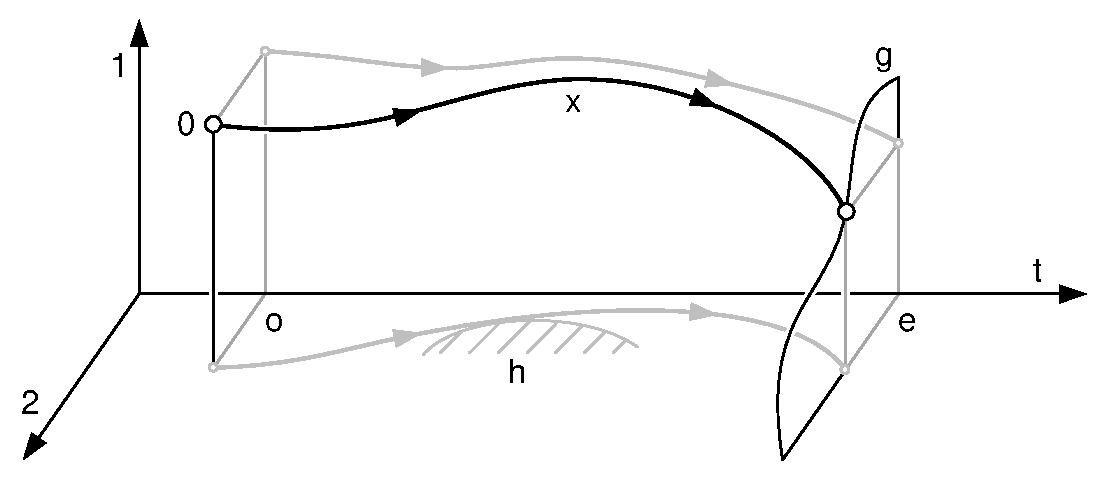
\includegraphics[width=1.\textwidth,clip, trim = 0cm 0cm 0cm 0cm]{pics/2_Darstellung_dynamische_Optimierung_endvorgabe.eps}
  	\caption[Example of an optimal trajectory]{Example of an optimal trajectory $\bs{x}^\ast (t)\in \mathbb{R}^2$ with end constraints $\bs{g}=\bs 0$ at a fixed final end time $t_f$ and inequality constraint $h\leq 0$ for $x_2$}
    \label{fig:dynamische_Optimierung_endvorgabe}
\end{figure}

\subsection{Problem Formulation for DAS and Automated Driving}\label{S:57.2.2}
Coming back to the automotive application, equation \eqref{equ:optimalsteuerungsproblem} of the previous section describes the dynamics of the vehicle. This state space model also includes the planar motion, either relative to some reference such as the lane center, see Sect. \ref{S:57.3.1.2}, or relative to a stationary origin, see Sect. \ref{S:57.3.3.4}. Undesired vehicle motion such as deviations from the lane center, detours, dangerous vehicle states (e.g., large slip angles), or uncomfortable jerks, e.g., caused by hectic steering actions will be penalized in the cost functional (1). The free space prediction between the generally moving obstacles can be described by the inequality constraints (4). And the end constraints (3) can be utilized to require that the optimized vehicle trajectory will be aligned to the road at the end of the optimization interval. As will be explained in Sect. \ref{S:57.5}, this final state plays an important role for the stability of the “replanning” algorithm, therefore special costs 
$V(\bs{x}(t_f), t_f)$ can be introduced in (1). 

\section{Solving the Optimal Control Problem}\label{S:57.3}
All known approaches to the OCP can be assigned to one of the following three principles, see e.g. \cite{diehl_fast_multipleshooting}.
\subsection{Approach I: Calculus of Variations}\label{S:57.3.1}
The classical approach to the OCP is \textit{calculus of variatins}, which delivers valuable insight in the solution. 

\subsubsection{Theoretical Background: Hamilton Equations}\label{S:57.3.1.1}

Static optimization problems can be tackled by \textit{differential calculus}. It is well known that the first derivative of a function $J(\bs p)$  is equal to zero at a minimum (or any other stationary point). For multivariate problems we can write $\nabla\!J(\bs x) = \bs 0$
which leads to a set of (algebraic) equations that the optimum 
$\bs{p}^\ast$ must satisfy. The extension to problems with equality constraints requires the method of so-called \textit{Lagrange-multipliers}, yielding first order necessary conditions for optimality.
Analogously for dynamic optimization, variational calculus requires that the first variation of the functional $J(\bs{u}(t))$
vanishes for the optimal control function $\bs{u}^\ast$
which is often written as $\delta J(\bs{u}(t))=0$. 

In order to incorporate the system dynamics in the OCP, which constitute (differential) equality constraints, we can also apply the Lagrange-multiplier method. This yields a set of differential equations, the so-called Hamilton equations:

%x ̇=f(x,u,t)	(57.1))
%λ ̇=-∂l/∂x-[∂f/∂x]^"T"  λ	(57.2))
%0=-∂l/∂u-[∂f/∂u]^"T"  λ

\begin{subequations} \label{equ:hamiltongl}
\begin{alignat}{1}
\dot {\bs x} 				&= \bs f(\bs x, \bs u, t) \label{equ:hamilton_dgl}\\
\dot {\bs \lambda} 	&= -\frac{\partial l}{\partial \bs x} - \left[\frac{\partial \bs f}{\partial \bs x}\right]^\T \bs \lambda \label{equ:hamilton_dgl_adj}\\
\bs 0     					   &= \,\,\,\,  \frac{\partial l}{\partial \bs u} + \left[\frac{\partial \bs f}{\partial \bs u}\right]^\T \bs \lambda \label{equ:hamilton_steuergleichung}
\end{alignat}
\end{subequations}

\begin{align}
\bs x(t_0) = \bs x_0 \label{equ:fester_anfangszustand}
\end{align}



They are \textit{first order necessary conditions} for our OCP, when there are no inequality constraints (4) involved. The function $\bs \lambda(t)$
constitutes the Lagrange-multipliers, here called \textit{co-states}. Besides the initial condition
\begin{align}
\bs x(t_0) = \bs x_0 \label{equ:fester_anfangszustand}
\end{align}
the optimal trajectory must fulfill the (algebraic)\textit{ transversality conditions}, depending on whether the end state $\bs x(t_f)$
is constraint by TODO (3) and/or the final time $t_f$ is given (see e.g. \cite{Lewis_OC}). 

The simplest condition requires a fixed end state $\bs x_f$ at a given end time  $t_f$
so that
\begin{align}
\bs x(t_f) = \bs x_f \label{equ:fester_endpunkt}
\end{align}
Either way, this results in a boundary value problem, which in general needs to be solved numerically. This so-called indirect approach is very accurate but not as flexible as the direct approach that we will introduce in Sect. \ref{S:57.3.2}. However, for simple OCPs the resultant boundary value problem can be solved analytically, leading to fast computable optimal trajectory primitives with broad applications (see Sect. \ref{S:57.4}).

\subsubsection{Example Application: Automated Lane Change}\label{S:57.3.1.2}
We will now apply the described method to the generation of optimal lane change primitives. The lateral motion across the road can be modelled as a triple integrator system with states $\bs x = [x_1, x_2, x_3]^\T$ , namely the position, the lateral velocity, and the lateral acceleration, respectively, all within the reference frame of some curve, see Fig. \ref{fig:polytraj}.
Then, the system dynamics are described by 
\begin{align}
	\dot{\bs x} = \bs f(\bs x, u) = [x_2, x_3, u ]^\T
	\label{equ:stateeqlc}
\end{align}
where $u$ represents the lateral jerk, which is the third derivative of the lateral position. We will now seek for the optimal system input $u^* (t)$  that transfers the integrator system from its initial state
\begin{align}
	\bs x(0) = \bs x_0 \label{equ:x_0}
\end{align}
to a given end state 
\begin{align}
\bs x(t_f) = \bs 0 \;, \label{equ:x_f}
\end{align}
at a given end time $t_f$. Amongst all trajectories we seek for the one that minimizes the integral of the jerk-square, that is
\begin{align}
	J &= %\int_{0}^{t_f}l(u(t)) {\rm d} t = 
	\int_{0}^{t_f}\frac{1}{2} u(t)^2 {\rm d} t \label{equ:integrator_J}
\end{align}
so that the movement feels most pleasant to the passengers. Notice that the final cost here has no influence on the solution due to the fixed end state, so that we can set $V=0$ in \eqref{equ:opt_funktional}.
With $\bs \lambda =\lambda_1, \lambda_2, \lambda_3]^\T$ , evaluating the so-called control equation \eqref{equ:hamilton_steuergleichung} we obtain
\begin{align}
	0 &=  u + \lambda_3 \quad \Rightarrow \quad u = -\lambda_3 \;. \label{equ:integrator_u}
\end{align}
The co-state equation \eqref{equ:hamilton_dgl_adj} yields
\begin{align*}
	\dot {\bs \lambda} = 
	\mtrx{c}{\dot{\lambda_1} \\ \dot{\lambda_2} \\ \dot{\lambda_3}}=
	 %-\frac{\partial H}{\partial \bs x} = %\mtrx{ccc}{0 & 0 & 0 \\ 1 & 0 & 0 \\ 0 & 1 & 0} \cdot \mtrx{c}{\lambda_1 \\ \lambda_2 \\ \lambda_3} =  
	\mtrx{c}{0 \\ \lambda_1 \\ \lambda_2}
\end{align*}
and therefore, we get
\begin{alignat}{3}
\nonumber
	\dot \lambda_1 &= 0 \quad  & &\Rightarrow &\quad \lambda_1(t) &= c_1 \\
\nonumber
	\dot \lambda_2 &= \lambda_1 & &\Rightarrow  & \lambda_2(t) &= c_1 t + c_2 \\
\label{equ:lambda_3}
	\dot \lambda_3 &= \lambda_2 & &\Rightarrow  & \lambda_3(t) &= \frac{1}{2}c_1 t^2 + c_2 t + c_3 \; , 
\end{alignat}
With $\lambda_3$ from \eqref{equ:lambda_3} it can be seen from \eqref{equ:integrator_u} that the optimal control input function is a third order polynomial with yet unknown integration constants $c_1, \ c_2,$ and $c_3$. Substituting $u(t)$ in the state equation \eqref{equ:stateeqlc} we find the optimal trajectory to 
\begin{alignat}{3}
	\dot x_3 &= -\lambda_3 \;\;  & &\Rightarrow &\;\; x_3(t) &= -\frac{1}{6}c_1 t^3 - \frac{1}{2}c_2 t^2 - c_3 t - c_4 \\
	\dot x_2 &= x_3 & &\Rightarrow  & x_2(t) &= -\frac{1}{24} c_1 t^4 - \frac{1}{6}c_2 t^3 - \frac{1}{2} c_3 t^2 - c_4 t - c_5 \\
	\dot x_1 &= x_2 & &\Rightarrow  & x_1(t) &= -\frac{1}{120} c_1 t^5 - \frac{1}{24} c_2 t^4 - \frac{1}{6}c_3 t^3 -\frac{1}{2}c_4 t^2 - c_5 t - c_6
	\label{equ:x_dots}
\end{alignat}

with additional integration constants $c_4,c_5,$ and $c_6$. To comply with the initial state \eqref{equ:x_0} and end constraint \eqref{equ:x_f} the integration constants need to be chosen accordingly. As \eqref{equ:lambda_3}-\eqref{equ:x_dots} are linear with respect to the constants this can be done by simple linear algebra, leading to the trajectory (a) in Fig. \ref{fig:polytraj} 
\\
Similarly, we can find the solution to the OCP with a free end state (and a free end time). In this case we require the end state to be as close to (and as soon at) the reference as possible by setting
\begin{align*}
V(x) &=k_1 x_1 (t_f)^2+k_2 x_2(t_f)^2 + k_3 x_3(t_f)^2 ,&& k_i>0\\
(V(x) &=k_t t_f+k_1 x_1 (t_f)^2+k_2 x_2(t_f)^2 + k_3 x_3(t_f)^2 ,&& k_i,k_t>0 )
\end{align*}
The new transversality conditions will only lead to a different end state and end time, see (b) and (c) in Fig \ref{fig:polytraj}. However, the optimal function class, that is the 5th-order polynomial, will stay the same.

\begin{figure}[h]
\centering
	\psfrag{t}[bc][bc]{$s(t)$}
	\psfrag{1}[cr][cr]{$x_1$}
	\psfrag{x}[cc][cc]{$\bs x^\ast$}
	\psfrag{0}[ct][ct]{$\bs x_0$}
	\psfrag{a}[cb][cb]{\scriptsize (a)}
	\psfrag{b}[ct][ct]{\scriptsize (b)}
	\psfrag{c}[ct][ct]{\scriptsize (c)}
	\psfrag{e}[bc][bc]{$t_f^\ast$}
	\centering
  	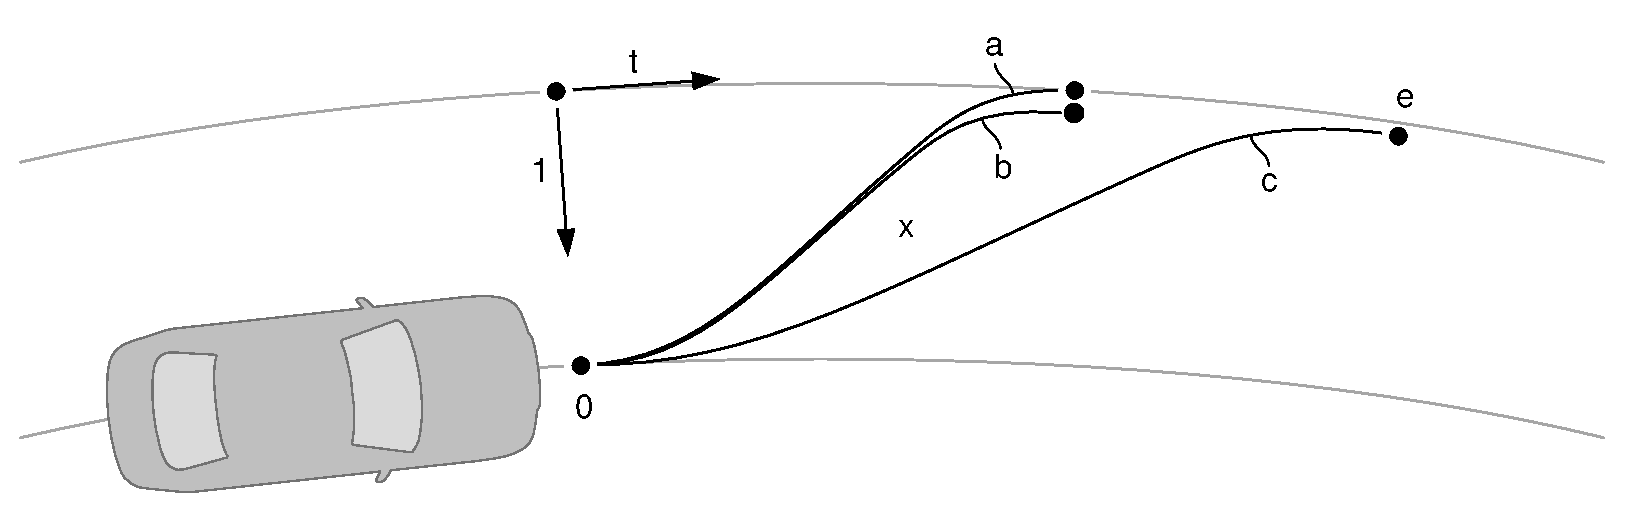
\includegraphics[width=.8\textwidth,clip, trim = 0cm 0cm 0cm 0cm]{6_Polytraj.eps}
  \caption{Optimal lane changes for (a) a given end time and end state; (b) a given end time and a free end state; (c) a free end time and a free end state}
    \label{fig:polytraj}
\end{figure}

\subsubsection{Further Readings}\label{S:57.3.1.3}

The previous calculations can be analogously carried out for the longitudinal movement, which leads to a very comfortable braking characteristic \cite{gutjahr2014automatic} %  (Gutjahr and Werling 2014). 
The longitudinal and lateral movements can also be combined by a regular local and temporal sampling of target states across and along the street. 
This leads to a reactive algorithm which prevents collisions with static and moving obstacles (Werling et al. 2012).\textbf{which???}
The variational approach was generalized to problems with input constraints, known as \textit{Pontryagin's minimum principle}.
 As for the vehicular application, it yields the shortest path connecting two poses of a vehicle with a limited turn radius \cite{dubins1957cml,reeds1990optimal,boissonnat1994note}. %(Dubins 1957; Reeds and Shepp 1990; Boissonnat et al. 1994). 
Even more involved is finding variational solutions to problems with state constraints such as the optimal braking application in Fig. \ref{fig:poly_mit_unb} \textbf{which???}(e.g., Bryson and Ho 1975).
Numerical solutions to the first order necessary conditions can be found by so-called indirect methods (see e.g.  \cite{Graichen2012} )% Graichen 2012) 
which provide very accurate results in general. Contrary to direct methods, as described in the sequel, they need to determine initial conditions for the co-states, which has made the applications unsuitable for an automotive online application yet.





\begin{figure}[ht]
\centering
% Generated using matlabfrag
% Version: v0.6.16
% Version Date: 04-Apr-2010
% Author: Zebb Prime
%
%% <text>
%
\providecommand\matlabtextA{\color[rgb]{0.000,0.000,0.000}\fontsize{10}{10}\selectfont\strut}%
\psfrag{016}[bc][bc]{\matlabtextA \xlabelX}%
\psfrag{017}[bc][bc]{\matlabtextA \xlabelT}%
\psfrag{018}[tc][tc]{\matlabtextA \ylabelA}%
\psfrag{019}[tc][tc]{\matlabtextA \ylabelV}%
%
%% </text>
%
%% <xtick>
%
\def\matlabfragNegXTick{\mathord{\makebox[0pt][r]{$-$}}}
%
\psfrag{000}[ct][ct]{\matlabtextA $0$}%
\psfrag{001}[ct][ct]{\matlabtextA $10$}%
\psfrag{002}[ct][ct]{\matlabtextA $20$}%
\psfrag{003}[ct][ct]{\matlabtextA $30$}%
\psfrag{004}[ct][ct]{\matlabtextA $40$}%
\psfrag{005}[ct][ct]{\matlabtextA $0$}%
\psfrag{006}[ct][ct]{\matlabtextA $1$}%
\psfrag{007}[ct][ct]{\matlabtextA $2$}%
\psfrag{008}[ct][ct]{\matlabtextA $3$}%
\psfrag{009}[ct][ct]{\matlabtextA $4$}%
%
%% </xtick>
%
%% <ytick>
%
\psfrag{010}[rc][rc]{\matlabtextA $-10$}%
\psfrag{011}[rc][rc]{\matlabtextA $-5$}%
\psfrag{012}[rc][rc]{\matlabtextA $0$}%
\psfrag{013}[rc][rc]{\matlabtextA $0$}%
\psfrag{014}[rc][rc]{\matlabtextA $10$}%
\psfrag{015}[rc][rc]{\matlabtextA $20$}%
%
%% </ytick>
\renewcommand{\matlabtextA}{\normalsize }
	\def\ylabelV{$x_2$ in $\unitfrac{m}{s}$}
	\def\ylabelA{$x_3$ in $\unitfrac{m}{s^2}$}
	\def\xlabelT{$t$ in $\unit{s}$}
	\def\xlabelX{$x_1$ in $\unit{m}$}
	\centering
  	
\includegraphics[width=1.\textwidth,clip, trim = 0cm 0cm 0cm 0cm]{6_Hamilton_constraint.eps}
  \caption{Minimal jerk-square minimal time stopping trajectories with acceleration constraint with $a\geq -10 \unitfrac{m}{s^2}$}
    \label{fig:poly_mit_unb}
\end{figure}



\subsection{Approach II: Direct Optimization Techniques}\label{S:57.3.2}


\subsection{	Theoretical Background: Finite Parameterization Approximation}\label{S:57.3.2.1}
Direct optimization is probably the most widely explored approach in model-predictive control. It approximates the dynamic optimization problem of the OCP to a static one, as the latter can be efficiently solved by well-established numerical solvers. The essence of this approach is a \textit{finite-dimensional parameterization} of the input, state, or output trajectory.
Here, we will introduce a very common method called single shooting. In a first step, we chose a finite dimensional parameterization of the input
\begin{align*}
	\bs{u}(t) = \bs{\psi}(t,\bar{\bs{u}}) = \bs{u}_i, \, t\in[t_i, t_{i+1}) \quad \text{und} \quad \bar{\bs{u}} = [\bs{u}_0, \bs{u}_1, \ldots, \bs{u}_{N-1}]^\T.
\end{align*}
such as a piecewise constant interpolation (see  Fig. \ref{fig:parametrisierte_nmpc}), a polynomial, or a spline. The input trajectory is therefore fully described by the finite parameter vector $\bar{\bs{u}}$. The system dynamics \eqref{equ:opt_systemdynamik} now read
\begin{align*}
	\dot{\bs{x}}(t) = \bs{f}(\bs{x}(t),\bs{\psi}(t,\bar{\bs{u}}),t), \quad &\bs{x}(t_0) = \bs{x}_0\; , 
\end{align*}
This constitutes an initial value problem, which can be solved by an ordinary differential equations solver. We denote the resultant trajectory by 
\begin{align*}
\bs{x}(t) = \bs{\phi}(t,\bar{\bs{u}}).
\end{align*}
Furthermore, it is standard practice that the inequality constraints are only required to hold at $N$ discrete equidistant points in time $t_i,i=1,\dots,N,$ so that the number of inequality constraints is also finite. 
Thus, the OCP was transformed to the following static optimization problem:\\
Minimize the cost function
\begin{subequations}
\begin{align}
J(\bs{\phi}(t,\bar{\bs{u}}),\bs{\psi}(t,\bar{\bs{u}}),t)) = 
	\int_{t_0}^{t_f} l(\bs{\phi}(t,\bar{\bs{u}}),\bs{\psi}(t,\bar{\bs{u}}),t)\,{\rm d} t + V(\bs{\phi}(t_f,\bar{\bs{u}}))
\label{equ:diroptcost}
\end{align}
subject to the equality and inequality constraints
\begin{align}
	 &\bs{g}(\bs{\phi}(t_f,\bar{\bs{u}}),t_f) = \bs{0} \label{equ:diropteqcon}\\ 	
	&\bs{h}(\bs{\phi}(t_i,\bar{\bs{u}}),\bs{\psi}(t_i,\bar{\bs{u}}))  \leq \bs{0},  \quad  i=0,\ldots,N \label{equ:diroptineqcon}\;. 
\end{align} 
\end{subequations}

Loosely speaking, for a first guess $\bar{\bs{u_0}}$ the system will be simulated in a “single shoot” for $t \in [0,t_f]$  starting from $x_0$. Then, the total costs J are evaluate as well as the constraints $\bs{g}$ and $\bs{h}$ in \eqref{equ:diroptcost}, \eqref{equ:diropteqcon}, and \eqref{equ:diroptineqcon}, respectively. These values are then fed back to a numerical solver, which repeats this procedure by a variation of $\bar{\bs{u}}$to conclude how to modify the parameter so that $J$ gets smaller without violating $\bs{g}=\bs{0}$ and $\bs{h}\leq\bs{0}$. When the solution does not significantly change any more or a certain number of iterations have been reached, the optimization will be terminated.



\begin{figure}[h]
\centering
	\psfrag{0}[cr][cr][1.0]{$\bs{x}_0$}
	\psfrag{1}[cb][cb][1.0]{$\bs{u}_0$}
	\psfrag{2}[cb][cb][1.0]{$\bs{u}_1$}
	\psfrag{3}[cb][cb][1.0]{$\bs{u}_2$}
	\psfrag{f}[cl][cl][1.0]{$\bs{x}(t_f)$}
	\psfrag{7}[cl][cl][1.0]{$g=0$}
	\psfrag{t}[ct][ct][1.0]{$t$}
	\psfrag{a}[ct][ct][1.0]{$0$}
	\psfrag{b}[ct][ct][1.0]{$t_f$}
	\psfrag{x}[cb][cb][1.0]{$\bs{x}(t) = \bs{\phi}(t,\bar{\bs{u}})$}
	\psfrag{u}[cb][cb][1.0]{$\bs{u}(t) = \bs{\psi}(t,\bar{\bs{u}})$}
 %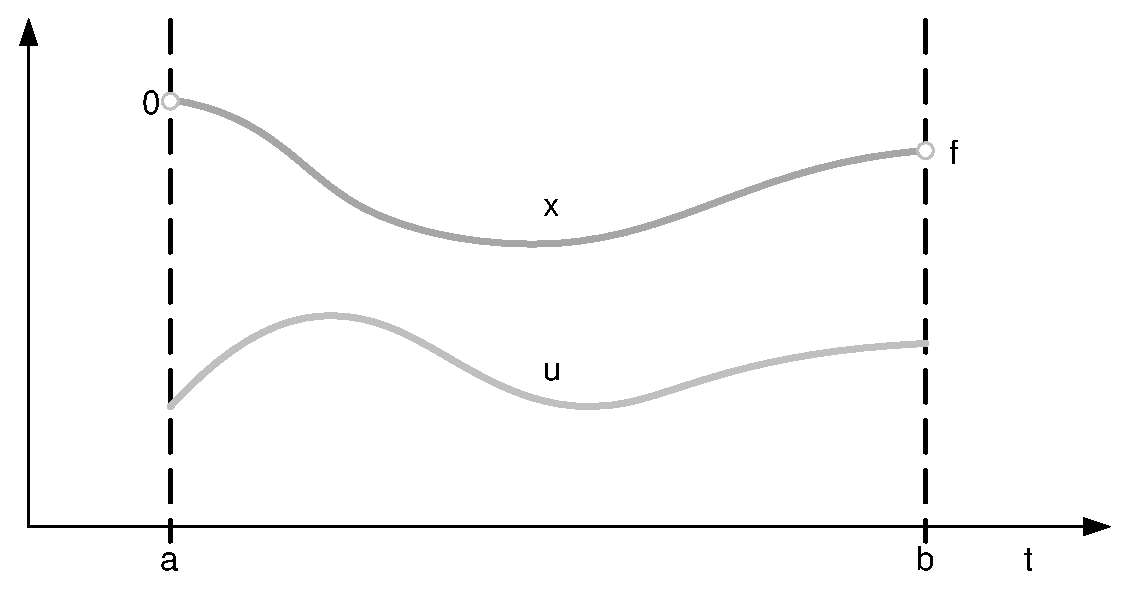
\includegraphics[width=0.5\textwidth,clip, trim = 0cm 0cm 0cm 0cm]{2_Darstellung_dynamische_Optimierung.eps}
%\hspace{.5cm}
 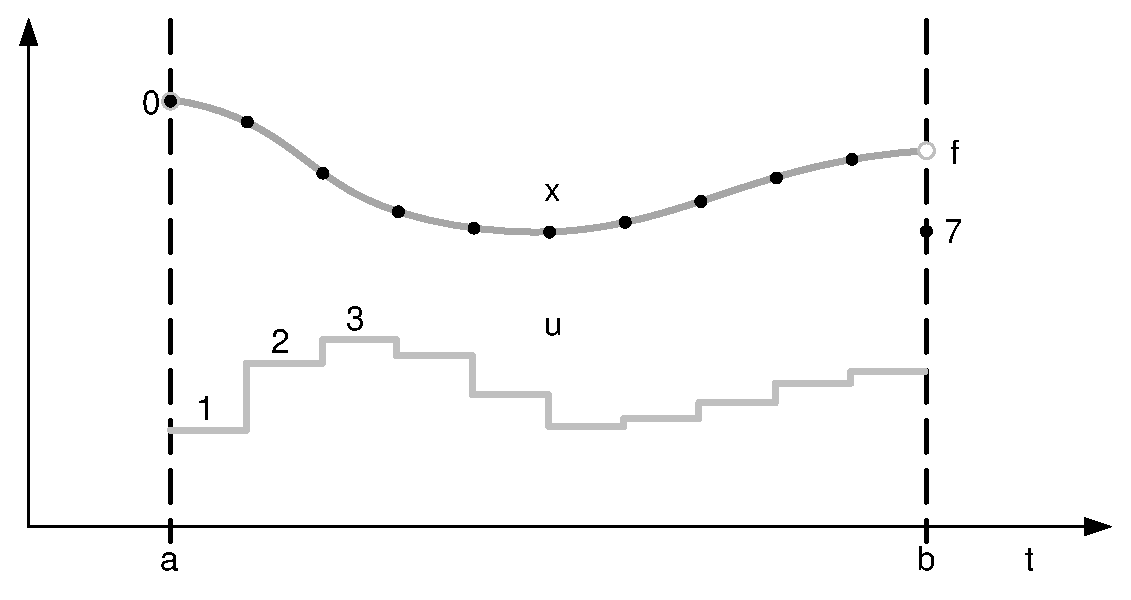
\includegraphics[width=1.0\textwidth,clip, trim = 0cm 0cm 0cm 0cm]{2_Darstellung_endliche_Parametrierung.eps}
	\caption[Finite parameterization of the input]{Finite parameterization of the input and sampling of the constraints \cite{papageorgiou2012optimierung}} 
	\label{fig:parametrisierte_nmpc}
\end{figure}


\subsubsection{Example Application: Emergency Obstacle Avoidance}\label{S:57.3.2.2}

The direct method will now be applied to a combined steering and braking maneuver as part of a possible future \emph{active safety} system \cite{werling2012cdc}. % (Werling and Liccardo 2012). 
For simplicity, we will approximate the vehicle dynamics by the static \emph{one-track model} with only two parameters, the wheel base l and the characteristic speed $v_\mathrm{ch}$. We then get
\begin{align}
\label{equ:thetadot}
\dot \theta &= \frac{v}{l \left[ 1 + \left[\frac{v}{v_{\text{ch}}}\right]^2\right]} \delta
\end{align}
where $\delta$ denotes the steering angle at the wheels, $v$ is the velocity, and $\theta$ describes the course angle of the vehicle in some stationary reference frame. To avoid discontinuities in the steering angle trajectory, we extend the model by
\begin{align*}
\dot \delta &= u
\end{align*}
so that the steering rate serves as the system input. We parameterize it by a \textit{piecewise constant} input
\begin{align*}
u(t)=\psi(t,\bar{\bs{u}}))=u_i, \quad  t \in [t_i,t_{i+1}) \quad \text{and} \quad \bar{\bs{u}} = [u_0,u_1,\dots,u_{N-1}]^\T
\end{align*}
with $N$ equidistant intervals.
Throughout the maneuver the brake should be engaged as much as physically reasonable and therefore it is required that the vehicle accelerations stay right on the \emph{friction ellipse}

\begin{align} \label{equ:ellipse}
\left[\frac{a_t}{c_t}\right]^2 + \left[\frac{a_n}{c_n}\right]^2 -1 = 0.
\end{align}
see Fig \ref{kammscherKreis}, where the lateral and longitudinal acceleration are given by $a_n=v \dot{theta}$ and $a_t=\dot{v}$.

% [Physical acceleration limits] \hspace{1.8cm} [System states]
\begin{figure}[h]%
\centering
    \psfrag{1}[rb][rb][1.0]{$a_t$}
    \psfrag{2}[cb][cb][1.0]{$a_n$}
    \psfrag{3}[lc][lc][1.0]{$c_t$}
    \psfrag{4}[ct][ct][1.0]{$c_n$}
    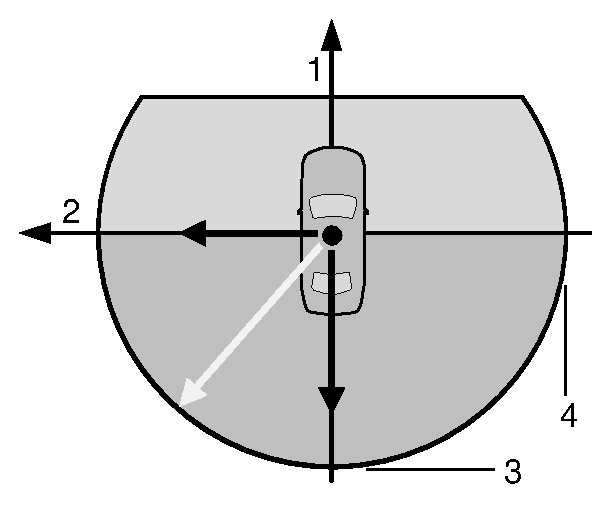
\includegraphics[width=0.5\textwidth,clip, trim = 0cm 0cm 0cm 0cm]{5_KammscherKreis}
    \caption[Physical acceleration limits]{Physical acceleration limits}
    \label{fig:kammscherKreis}
\end{figure}%

Solving the equation for $a_n$ leads to the longitudinal dynamics 
\begin{align} \label{equ:replacement}
	\dot v = -c_t \sqrt{1-[v\dot\theta / c_n]^2}
\end{align}

of the full braking vehicle, where $\dot{\theta}$ must be replaced by the expression in \eqref{equ:thetadot}. 
In other words, the steering angle $\delta$ directly influences how much the vehicle can slow down. 
Hence, there is no need to optimize the braking power by a separate optimization variable. 
Next, the planar vehicle motion will be modelled. 
Choosing street relative coordinates bears some calculative advantages over Cartesian coordinates $[x_1,x_2]$ in the cost functional. We therefore describe the vehicle motion (approximately) by

\begin{subequations} \label{equ:dgl_mdl_nmpc_2}
\begin{align}
\label{equ:d_r_dot}
\dot d_r &= v \sin(\theta - \theta_r) \\
\dot \theta_r &= v \cos(\theta - \theta_r)\kappa_r(s_r) \\
\label{equ:s_r_dot}
\dot s_r &= v,
\end{align}
\end{subequations}

with the curve offset $d_r$ with respect to the center of the lane, the curve’s orientation $\theta_r$ and curvature $\kappa_r$  as well as the curve length parameter $s_r$.
All variables referred to the vehicle projection point on the curve, see Fig. \ref{fig:systemStates}. The set of ordinary differential equations \eqref{equ:thetadot}-\eqref{equ:s_r_dot} is particularly non-stiff so that it can be integrated by the simple first order Runge-Kutta scheme.
% [Physical acceleration limits] \hspace{1.8cm} [System states]
\begin{figure}[h]%
\centering
\psfrag{1}[tc][tc][1.0]{$s_r$}
    \psfrag{2}[rb][rb][1.0]{$\kappa_r(s_r)$}
    \psfrag{3}[lb][lb][1.0]{$d_r$}
    \psfrag{4}[rb][rb][1.0]{$[x_1, x_2]$}
    \psfrag{5}[lt][lt][1.0]{$v$}
    \psfrag{6}[c][c][1.0]{$\theta$}
    \psfrag{7}[lt][lt][1.0]{$\theta_r$}
    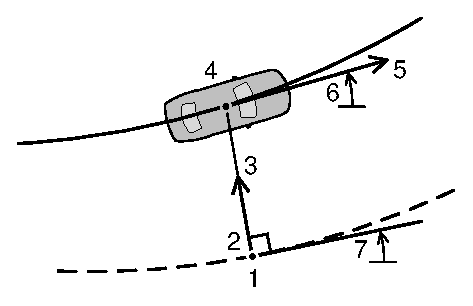
\includegraphics[width=0.5\textwidth,clip, trim = 1.5cm 0cm 0cm 0cm]{5_vehicleAndReferenceCurveStates.eps}
    \caption[System states]{System states relative to the road center}
    \label{fig:systemStates}
\end{figure}%
For the costs we choose
\begin{align}
\label{equ:integralcosts}
J = \int_{t_0}^{t_f}{ \left[ u^2 + k_1 (\theta-\theta_r)+k_2(\kappa - \kappa_r) \right] }dt \quad \text{with} \quad  \kappa = \frac{\delta}{l \left[ 1 + \left[\frac{v}{v_{\text{ch}}}\right]^2\right]}
\end{align}
to avoid excessive steering rates as well as large deviations from the reverence curve heading and curvature. The costs can be simply calculated by integrating the running costs $l$ in parallel to the system dynamics, that is $\dot{J}=l(\bs{x},u)$.

To formulate inequality constraints that prevent the vehicle from colliding with the obstacle, for a given trajectory we define the point in time $t_{d,\mathrm{min}}$, when the (possibly moving) obstacle is the closest to the vehicle. 
The projection of the distance vector $\bs{\xi}^\T(d_r(t_{d,\mathrm{min}}),s_r(t_{d,\mathrm{min}},t_{d,\mathrm{min}})$ to the obstacle onto the normal vector $\bs{n}\left(\theta(t_{d,\mathrm{min}})\right)$ of the vehicle course has to yield some safety clearance $d_\mathrm{safety}$. Therefore

\begin{align*}
\bs{\xi}^\T\left(d_r(t_{d,\mathrm{min}}),s_r(t_{d,\mathrm{min}})\right)^\T \ \cdot \bs{n}\left(\theta(t_{d,\mathrm{min}})\right) +d_\mathrm{safety} \leq 0
\end{align*}

has to hold, when we want to force the vehicle to pass on the left side of the obstacle. 
Also, we require the optimal trajectory to stay within the left lane boundaries, which can be expressed as

\begin{align*}
d_r(t_i) - \left[ d_max \right] \leq 0 \quad i=1,\dots,N.
\end{align*}
The resultant so-called \emph{nonlinear program} executes with $N=20, t_f=2.0\mathrm{s}$ , and an initial guess of $\bar{\bs{u}}_0=\bs{0}$ in approximately 100ms  on an i5-520M (2.4 GHz). A pedestrian example is shown in Fig.\ref{fig:fussgaenger_draufsicht}. As can be seen, the vehicle uses the full friction potential (bottom left) while braking and evading the pedestrian (black dot within gray safety margin) without leaving the given lane boundary (dotted line).
%[Combined braking and steering]
\begin{figure}[h]
	\centering
	% Generated using matlabfrag
% Version: v0.6.16
% Version Date: 04-Apr-2010
% Author: Zebb Prime
%
%% <text>
%
\providecommand\matlabtextA{\color[rgb]{0.000,0.000,0.000}\fontsize{10}{10}\selectfont\strut}%
\psfrag{000}[bc][bc]{\matlabtextA $t=2\unit{s}$}%
\psfrag{001}[bc][bc]{\matlabtextA $t=0.8\unit{s}$}%
\psfrag{002}[bc][bc]{\matlabtextA $t=0.25\unit{s}$}%
\psfrag{003}[bc][bc]{\matlabtextA $t=0\unit{s}$}%
%
%% </text>
	\renewcommand{\matlabtextA}{\scriptsize}
	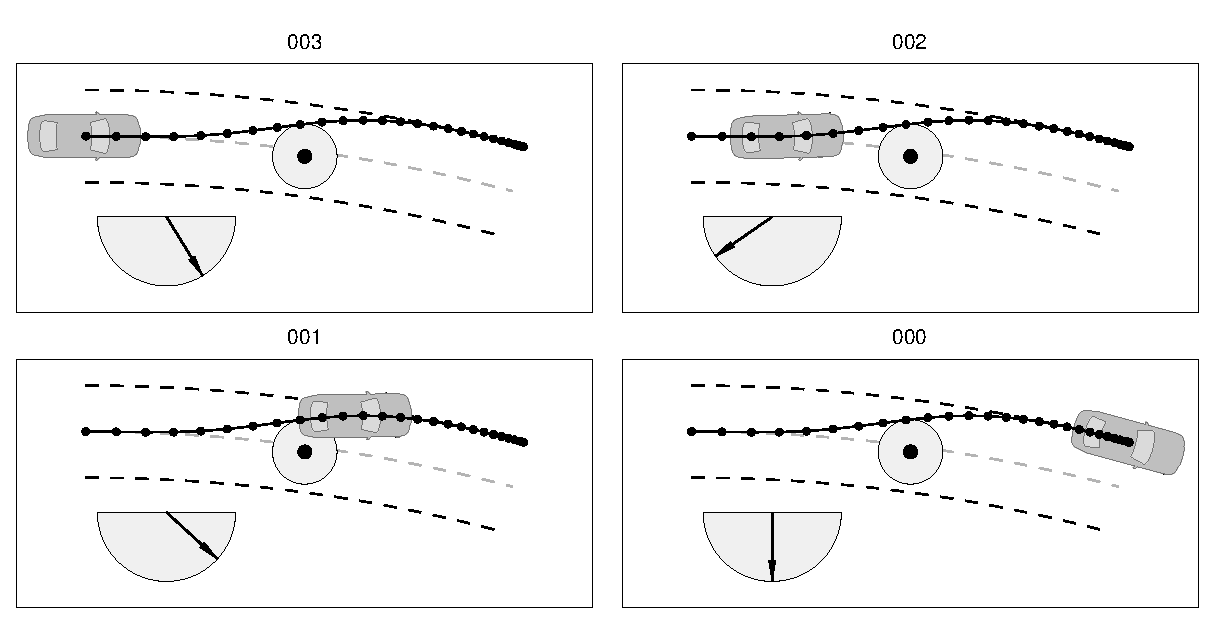
\includegraphics[width=1.0 \linewidth,trim = 0cm 0cm 0cm 0cm]{5_AuswertungSingleshooting_szene.eps}		
	%def\xlabel{$t$ in \unit{s}}
    \caption[Combined braking and steering]{Automatic obstacle avoidance with combined braking and steering at the friction limit; the safety margin $d_\mathrm{safety}$  is shown as a grey circle around the stationary pedestrian depicted as a black dot; the lane boundaries given by $d_\mathrm{max}$  are drawn as grey dotted lines.}
    \label{fig:fussgaenger_draufsicht}
\end{figure}


\begin{figure}	
\centering
	\def\xlabel{$t$ in $\unit{s}$}
	\def\ylabelA{$v$ in $\unitfrac{m}{s}$}	
	\def\ylabelB{$\delta$ in $\unit{rad}$}	
	\def\ylabelC{$u_1$ in $\unitfrac{rad}{s}$}
	\def\ylabelD{$a_t$ in $\unitfrac{m}{s^2}$}	
	\def\ylabelE{$a_n$ in $\unitfrac{m}{s^2}$}
	% Generated using matlabfrag
% Version: v0.6.16
% Version Date: 04-Apr-2010
% Author: Zebb Prime
%
%% <text>
%
\providecommand\matlabtextA{\color[rgb]{0.000,0.000,0.000}\fontsize{10}{10}\selectfont\strut}%
\psfrag{020}[tc][tc]{\matlabtextA \xlabel}%
\psfrag{021}[tc][tc]{\matlabtextA \ylabelA}%
\psfrag{022}[tc][tc]{\matlabtextA \ylabelD}%
\psfrag{023}[tc][tc]{\matlabtextA \ylabelE}%
\psfrag{024}[tc][tc]{\matlabtextA \ylabelB}%
\psfrag{025}[tc][tc]{\matlabtextA \ylabelC}%
%
%% </text>
%
%% <xtick>
%
\def\matlabfragNegXTick{\mathord{\makebox[0pt][r]{$-$}}}
%
\psfrag{000}[ct][ct]{\matlabtextA $0$}%
\psfrag{001}[ct][ct]{\matlabtextA $0.5$}%
\psfrag{002}[ct][ct]{\matlabtextA $1$}%
\psfrag{003}[ct][ct]{\matlabtextA $1.5$}%
\psfrag{004}[ct][ct]{\matlabtextA $2$}%
%
%% </xtick>
%
%% <ytick>
%
\psfrag{005}[rc][rc]{\matlabtextA $0$}%
\psfrag{006}[rc][rc]{\matlabtextA $10$}%
\psfrag{007}[rc][rc]{\matlabtextA $20$}%
\psfrag{008}[rc][rc]{\matlabtextA $-10$}%
\psfrag{009}[rc][rc]{\matlabtextA $0$}%
\psfrag{010}[rc][rc]{\matlabtextA $10$}%
\psfrag{011}[rc][rc]{\matlabtextA $-10$}%
\psfrag{012}[rc][rc]{\matlabtextA $0$}%
\psfrag{013}[rc][rc]{\matlabtextA $10$}%
\psfrag{014}[rc][rc]{\matlabtextA $-1$}%
\psfrag{015}[rc][rc]{\matlabtextA $0$}%
\psfrag{016}[rc][rc]{\matlabtextA $1$}%
\psfrag{017}[rc][rc]{\matlabtextA $-1$}%
\psfrag{018}[rc][rc]{\matlabtextA $0$}%
\psfrag{019}[rc][rc]{\matlabtextA $1$}%
%
%% </ytick>
	\renewcommand{\matlabtextA}{\normalsize }
  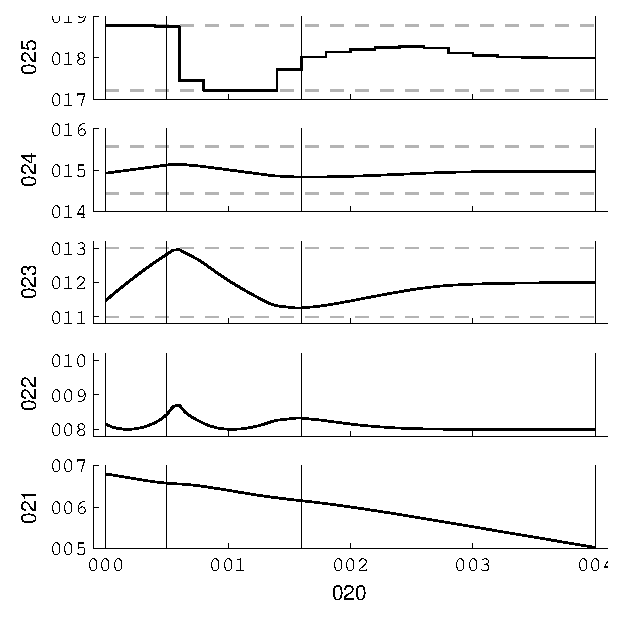
\includegraphics[width=1.0 \linewidth,trim = 0cm 0cm 0cm 0cm]{5_AuswertungSingleshooting_signals.eps}
    \caption[Signalverläufe bei kombiniertem Bremsen und Ausweichen]{\textbf{Figure nicht ist nicht im Word Dokument}Signalverläufe zu Abb.\,\ref{fig:fussgaenger_draufsicht} mit optimaler Steuerung $u_1$, Lenkwinkel $\delta$,  Quer- und Längsbeschleunigung $a_t, a_n$ sowie Geschwindigkeit $v$; Die vertikalen Linien markieren die Zeitpunkte der Draufsichten, die horizontalen gestrichelten Linien die Nebenbedingungen \cite{werling2012cdc}.}
    \label{fig:fussgaenger_draufsicht_signale}
\end{figure}

\subsubsection{Further Readings}\label{S:57.3.2.3}

Single shooting has been intensively studied for many vehicular applications such by \cite{kelly2003reactive,falcone2007linear,howard2007optimal,Yoon2009,gerdts2009generating, park2009obstacle}.% (Kelly and Nagy 2003), (Falcone et al. 2007), (Howard and Kelly 2007), (Yoon et al. 2009), (Gerdts et al. 2009), and (Park et al. 2009). 
Nevertheless, many other numerical methods exist such as \emph{multi-shooting} (Bock and Plitt 1984)\textbf{which???} and \emph{collocation} (Hargraves and Paris 1987)\textbf{which???} that might gain in importance in the future when dealing with instable vehicle models in challenging driving conditions. 
As for all direct optimization methods they lead to a static optimization problem, which can be most successfully solved by \emph{sequential quadratic programming} (SQP) techniques or \emph{interior point methods} (IP), see \cite{nocedal2006numerical}.%(Nocedal and Wright 2006).
As an alternative to a finite parameterization of the input, for flat systems \cite{rouchon1993flatness1}\textbf{orflatness2???}%(Rouchon et al. 1993) 
the flat output can be parameterized instead \cite{kang2012online},%(Kang 2012),
 which has been successfully demonstrated in complex inner-city scenarios by \cite{ziegler2014trajectory}. %(Ziegler et al. 2014).
In order to reduce the computational effort to a few milliseconds, (Falcone et al. 2007)\textbf{which???} and \cite{carvalho2013predictive},%(Carvalho et al. 2013),
for instance, approximated the formulation of trajectory optimization as a \emph{quadratic problem} (QP). This way no iterations are required as the solution can be found in a single step.

\subsection{Approach III: Dynamic Programming}\label{S:57.3.3}
Certain tasks such as parking in several moves or finding the way through multiple moving obstacles are \emph{combinatorial} (non-convex) \emph{problems}. They cannot be tackled by (local) direct optimization methods as the latter rely on an initial solution. However, \emph{dynamic programming} is a principle from \cite{bellmann_DP}%(Bellman 1954)
 that significantly reduces the computational burden of these combinatorial problems, so that the \textit{global optimum} can be efficiently obtained. It is therefore no surprise that it can be found in numerous (discrete) optimization algorithms.


\subsubsection{Theroetical Backgorund: Bellman’s Principle of Optimality}\label{S:57.3.3.1}
Richard \emph{Bellman’s principle of optimality} states:

\begin{mydef}
“An optimal policy has the property that whatever the initial state and initial decision are, the remaining decisions must constitute an optimal policy with regard to the state resulting from the first decision.” 
\end{mydef}

In other words, an optimal trajectory is composed of optimal sub-trajectories. This can be understood by looking at Fig. \ref{fig:Darstellung_Bellmanprinzip}, which shows the optimal trajectory $\bs{x}^* (t)$ in black connecting $\bs{x_0}$ with $\bs{x_f}$. The sub-trajectory (b), bringing $\bs{x^*} (t_1 )$ to $\bs{x_f}$, must be optimal, too. Otherwise, there would be another sub-trajectory (c) (grey), that would lead to a better total trajectory (a)+(c), which is contrary to the optimal trajectory $x^* (t)$ comprising (a)+(b).

	%[Bellman's principle of optimality]
%\section*{Dynamic Programming}
\begin{figure}[h]
	\psfrag{0}[cr][cr][1.0]{$\bs x_0$}
	\psfrag{f}[cl][cl][1.0]{$\bs x_f$}
	\psfrag{t}[ct][ct][1.0]{$t$}
	\psfrag{a}[ct][ct][1.0]{$0$}
	\psfrag{b}[ct][ct][1.0]{$t_f$}
	\psfrag{e}[lb][lb][1.0]{(a)}
	\psfrag{y}[tr][tr][1.0]{$\bs x^\ast(t)$}
	\psfrag{z}[br][br][1.0]{(b)}
	\psfrag{n}[tl][tl][1.0]{(c)}
	\psfrag{x}[cb][cb][1.0]{$\bs x^\ast(t_1)$}
	\psfrag{g}[ct][ct][1.0]{$t_1$}
	\centering
 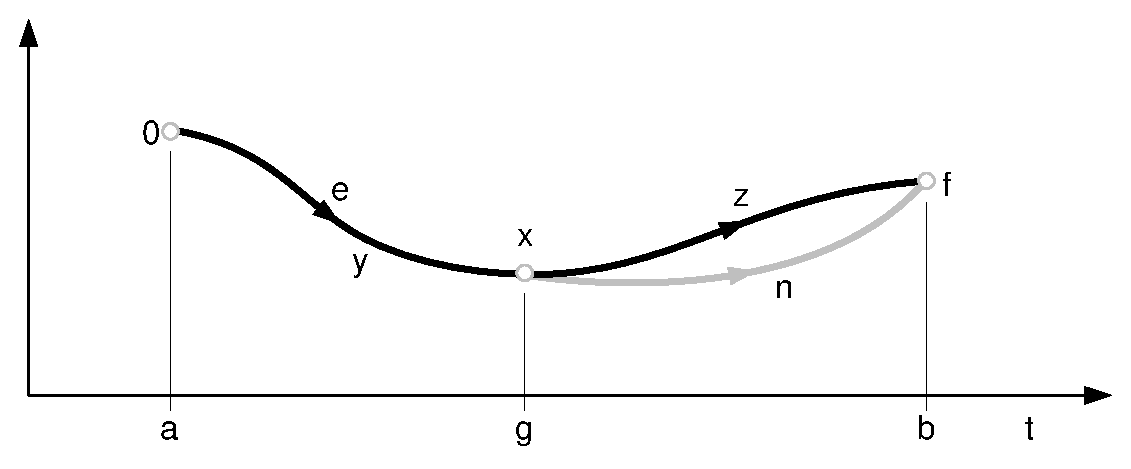
\includegraphics[width=1.0\textwidth,clip, trim = 0cm 0cm 0cm 0cm]{7_Darstellung_Bellmanprinzip.eps}
	\caption[Bellman’s Principle of Optimality]{Illustration of Bellman’s Principle of Optimality} 
	\label{fig:Darstellung_Bellmanprinzip}
\end{figure} 

The largest practical benefit from this principle is received when time-discretizing the OCP. We therefore consider the time-discrete process
\begin{align} \label{equ:diskreter_prozess}
	\bs x(k+1) = \bs f(\bs x(k), \bs u(k), k), \quad k=0,\ldots, k_f-1
\end{align}
and seek for the optimal steering sequence $\bs{u}^\ast (k)$ that minimizes the cost function
\begin{align}
	J = \sum_{k=0}^{k_f-1} l(\bs x(k), \bs u(k),k) \;. \label{equ:diskrete_kosten} %+ V(\bs x(k_f)) 
\end{align}

Notice, that constraints can be easily incorporated in \eqref{equ:diskrete_kosten} by setting the costs $l=\infty$ when the equality or inequality equations are violated.
A basic element of dynamic programming is memorizing the costs of sub-trajectories. Therefore, we define the so-called \emph{cost-to-go}

\begin{align*}
	G = \sum_{\kappa = k}^{k_f-1} l(\bs x(\kappa), \bs u(\kappa),\kappa) % + V(\bs x(k_f))
\end{align*}
(notice the difference between $\kappa$ and $k$), which incur when going from an intermediate state $x(k)$ all the way to $k_f$.\\
At this point, it should be noticed that the minimal cost-to-go, denoted by $G^\ast$, is nearly as good as the solution $u^\ast$ itself, as will be seen later. The minimal cost-to-go can be found in \emph{Bellman’s Recursion Formula}
\begin{mydef}
\begin{align*}
 G^\ast(\bs x(k),k) = \min_{\bs u(k)}\{\,l(\bs x(k), \bs u(k), k) + G^\ast(\bs f(\bs x(k), \bs u(k), k), k+1)\,\} \, ,
\end{align*}
\end{mydef}

which can be derived from the principle of optimality in a few steps. 
In words, it relates the minimal cost-to-go of the state $\bs{x}(k)$ at the $k^\mathrm{th}$  step, namely $G^\ast (\bs{x}(k),k)$, to the subsequent minimal cost-to-go $G^\ast (f(\bs{x}(k),\bs{u}(k),k),k+1)$ in consideration of the best choice of the possible inputs $\bs{u}(k)$ with its associated stage cost $l(\bs{x}(k),\bs{u}(k),k)$. The formula is used to break down the multi-staged OCP into simpler single-staged optimizations, which numerous algorithms exploit it to their advantage.

\subsubsection{Value Iteration}\label{57.3.3.2}


A very suitable and likewise simple algorithm to solving OCPs is \emph{value-iteration} that we will present in its backwards form. 
We assume that the system input can only take discrete values from a given set, which depends on the current state and the current time, that is $\bs u(k) \in \mathcal U(\bs x(k),k)$. 
The set ensures that the input will transfer the system from one discrete state $\bs x(k) \in \mathcal X(k)$ to the next. We therefore get a multi-stage decision process, such as the simple example in  Fig. \ref{fig:dynamische_programmierung_veranschaulichung} with three discrete states in each time step (except for the goal state $\bs{x}_f$). 

%[Discrete decision process]
\begin{figure}[h]
	\psfrag{0}[tc][tc][1.0]{0}
	\psfrag{1}[tc][tc][1.0]{1}
	\psfrag{2}[tc][tc][1.0]{2}
	\psfrag{3}[tc][tc][1.0]{3}
	\psfrag{4}[tc][tc][1.0]{$k_f$}
	\psfrag{5}[tc][tc][1.0]{$x(0) = x_0$}
	\psfrag{6}[bc][bc][1.0]{$x(k_f) = x_f$}
	\psfrag{t}[bc][bc][1.0]{$k$}
	\psfrag{o}[bl][bl][1.0]{$x^\ast(k)$}
	\psfrag{x}[bl][bl][1.0]{$x$}
	\psfrag{u}[tr][tr][1.0]{$u^\ast(0)$}
	\psfrag{g}[b][b][1.0]{$8$}
	\psfrag{a}[b][b][1.0]{$6$}
	\psfrag{b}[b][b][1.0]{$5$}
	\psfrag{c}[b][b][1.0]{$8$}
	\psfrag{s}[b][b][1.0]{$10$}
	\psfrag{v}[b][b][1.0]{$9$}
	\psfrag{d}[b][b][.7]{$2$}
	\psfrag{e}[b][b][.7]{$4$}
	\psfrag{f}[b][b][.7]{$1$}
	\psfrag{h}[b][b][.7]{$6$}
	\psfrag{i}[b][b][.7]{$5$}
	\psfrag{j}[b][b][.7]{$8$}
	\psfrag{m}[tr][tr][1.0]{$\min$}
	\psfrag{k}[b][b][.7]{$3$}
	\psfrag{l}[b][b][.7]{$5$}
	\psfrag{n}[b][b][.7]{$6$}
	\psfrag{p}[br][br][.7]{$1$}
	\psfrag{q}[br][br][.7]{$4$}
	\psfrag{r}[b][b][.7]{$3$}
	\psfrag{z}[b][b][1.0]{$11$}
	\psfrag{y}[tr][tr][1.0]{$\argmin{}$}
	\centering
  	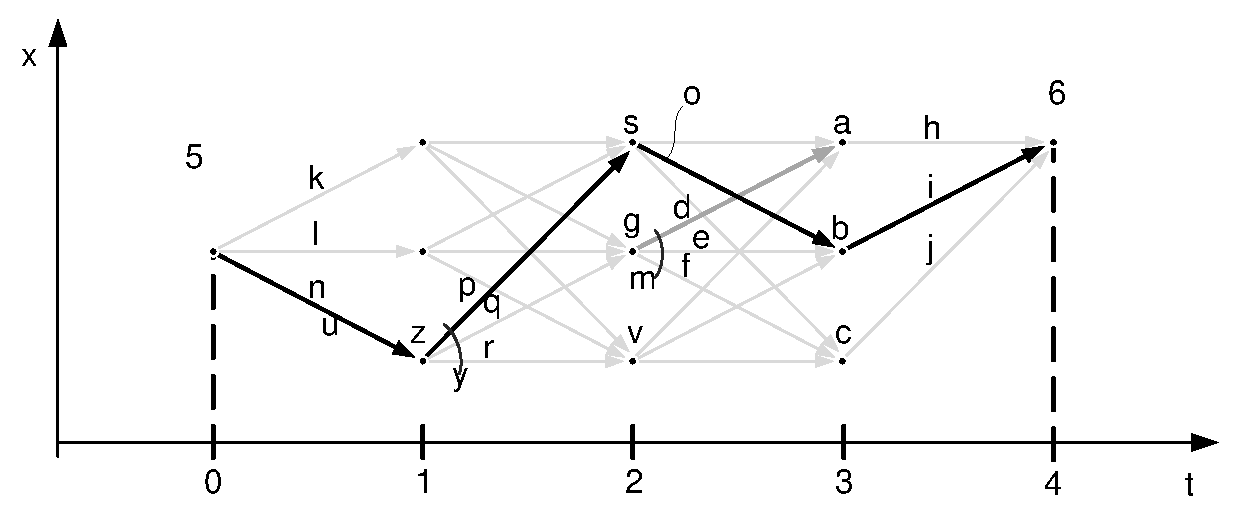
\includegraphics[width=0.98\textwidth,clip, trim = 0cm 0cm 0cm 0cm]{7_dynamische_programmierung_veranschaulichung.eps}
	\caption[Discrete decision process]{Discrete decision process with the optimal trajectory}
	\label{fig:dynamische_programmierung_veranschaulichung}
\end{figure} 

Even though the naive approach of evaluating all $3^3 = 27$ possibilities would here be feasible, this procedure is clearly prohibitive for realistically sized problems due to an exponential runtime of $\mathcal O(m^{k_f})$, where $m$ is the number of state transitions and $k_f$ the optimization horizon. 
However, we can apply the recursion formula, start with the last stage $k=k_{f-1}$, and work our way back to the first step. 
In doing so we calculate the optimal cost-to-go of every state of each stage by contemplating all possible transients and memorize it. 
This way it can be accessed when evaluating the optimal cost-to-go of the previous stage. Every stage can be done in $\mathcal O(m n)$, where $m$ and $n$ equals the number of its inputs and states. 
This adds up to a total runtime of $\mathcal O(m n k_f)$, which is only linear in the length of the optimization horizon. Fig. \ref{alg:valueiteration} summarizes the algorithm.

%\begin{figure}[h]
%  \caption[Value Iteration]{Value-iteration algorithm}

\begin{algorithm}
  \caption[Value Iteration]{Value-iteration algorithm}

 \begin{algorithmic}[1]

	%\FORALL{$\bs x \in \mathcal X(k_f-1)$}
%\STATE $G(\bs x) \leftarrow \infty$
%\ENDFOR
	\STATE $G^\ast(\bs x_f,k_f) \leftarrow 0$
	\FOR {$k=k_f-1$ \TO $0$}
		\FORALL{$\bs x \in \mathcal X$}
			\STATE $G^\ast(\bs x(k),k) = \underset{\bs u(k)}{\min}\{\,l(\bs x(k), \bs u(k), k) + G^\ast(\bs f(\bs x(k), \bs u(k), k),k+1)\,\}$
		\ENDFOR
	\ENDFOR
 \label{alg:valueiteration}

 \end{algorithmic}
 \end{algorithm}
%\end{figure}

The optimal input and state sequence $\bs{u}^\ast (k)$ and $\bs{x}^\ast (k)$ can now be found by an efficient forward search starting at $\bs{x}_0$ and alternating 

\begin{align} \label{equ:navigation_function}
\bs u^\ast(k) = \argmin{\bs u(k)}\{\,l(\bs x(k), \bs u(k), k) + G^\ast(\bs f(\bs x(k), \bs u(k),k), k+1)\,\}
\end{align}
and \eqref{equ:diskreter_prozess} for every stage to the end, see black arrows in  Fig. \ref{fig:dynamische_programmierung_veranschaulichung}.





\subsubsection{Example Application: Optimal Overtaking}\label{S:57.3.3.3}

A simplified problem setup and its solution can be found in Fig. \ref{fig:dynamische_programmierung_veranschaulichung}.
Here, the lateral motion is optimized, so that the car can proceed at a constant speed without getting too close to the other vehicles. 
The system state comprises of only the lateral position and velocity, hence 
$\bs{x}(k)=\left[d(k),v_\mathrm{lat}(k)\right]^\T$ , which is discretized with $\Delta d=0.5 \mathrm{m}$  and $\Delta v_\mathrm{lat}  =0.5\mathrm{m/s}$  at $t_k=k\cdot \Delta t$ with $k=1,\dots,10$ and $\Delta t=1.0 \mathrm{s}$ . Furthermore, the input set $\mathcal{U}$, i.e., all lateral acceleration profiles, is chosen as a first order polynomial with $-10.0\mathrm{m/s^2} <u(t)< 10.0\mathrm{m/s^2}$. And lastly, the stage costs are defined as

\begin{align*}
l \left(\bs{x}(k),u(k),k\right) = \int_{t_k}^{t_k+\Delta t}{u(t) dt}+k\left[d(k)-d_\mathrm{nearest}(k)\right]^2 +C_\mathrm{collision}\left(\bs{x}(k),u(k),k\right)
\end{align*}
with $k=1.0$, where $d_\mathrm{nearest}(k)$ denotes the lateral coordinate of the lane center closest to $d(k)$. 
The cost term $C_\mathrm{collision} \left(x(k),u(k),k\right)$ equals to zero if the vehicle does not collide within the interval $\left[t_k,t_k+\Delta t\right]$ and else equals to infinity. 
Due to the few system states with their coarse discretization, the (global) solution is found within a few milliseconds.

%[Dynamic programming example]
\begin{figure}[h]
	\psfrag{0}[l][l][.7]{0}
	\psfrag{O}[t][t][.7]{0}
	\psfrag{1}[t][t][.7]{1}
	\psfrag{2}[t][t][.7]{2}
	\psfrag{3}[t][t][.7]{3}
	\psfrag{4}[t][t][.7]{4}
	\psfrag{5}[t][t][.7]{5}
	\psfrag{6}[t][t][.7]{6}
	\psfrag{7}[t][t][.7]{7}
	\psfrag{8}[t][t][.7]{8}
	\psfrag{9}[t][t][.7]{9}
	\psfrag{a}[t][t][.7]{10}
	\psfrag{t}[t][t][1.0]{$k$}
	\psfrag{u}[r][r][1.0]{$u$}
	\psfrag{v}[r][r][1.0]{$v_\text{lat}$}
	\psfrag{d}[r][r][1.0]{$d$}
	\centering
	\centering
  	\includegraphics[width=0.98\textwidth,clip, trim = 0cm 0cm 0cm 0cm]{dp_example.eps}
	\caption[Dynamic programming example]{Dynamic programming example}
	\label{fig:dynamische_programmierung_veranschaulichung}
\end{figure} 


\subsubsection{Further Readings}\label{S:57.3.3.4}
The presented value iteration scheme is especially suited for structured dynamic environments as shown by \cite{zieg09spatemp},%(Ziegler et al. 2009),
\cite{McNaughton2011diss},%(McNaughton 2011), 
as well as \cite{Gu2012}.%(Gu and Dolan 2012). 
As can be seen in Fig. \ref{fig:lattice_strasse}, for natural, human like trajectories it is most advantageous to align the sampling along and across the road course. The costs usually penalize not only jerky, accelerant movements, and the approximation to obstacles, but also deviations from the desired road center. 
As opposed to that, in unstructured environments, such as parking lots, there is no preferred direction, so that the sampling uniformly covers the $[x,y]$ plane as shown in  Fig. \ref{fig:lattice}. 
As static obstacles dominate the problem, temporal aspects are usually neglected meaning that it is not important at what time a location is visited by the vehicle (see \cite{montemerlo2008junior},%(Montemerlo et al. 2008), 
\cite{zieglerIV08},%(Ziegler et al. 2008), 
\cite{pivtoraiko2009differentially},%(Pivtoraiko 2009),
\cite{likhachev2009planning},%(Likhachev and Ferguson 2009),
\cite{dolgov2010path}).% (Dolgov et al. 2010)). 
This drastically simplifies the preeoblem, however, value iteration cannot be applied anymore due to the loss of the processing sequence given by $k$ (the decision graph becomes cyclic). Therefore, a substitute order needs to be chosen, one that still leads to the optimum: Investigating the state (expanding the node) with the lowest cost-to-come leads to \emph{Dijkstra's algorithm}, unlike considering the state with the lowest (under)estimate on the total cost, which results in \emph{A* algorithm}, an informed search.
 The latter is especially efficient in unstructured environments, as the costs are dominated by the covered distance, which can be well estimated by the Euclidean distance (the so-called heuristic), see \cite{bertsekas2007}.%(Bertsekas 1995).


%[State lattice for unstructured environments]
\begin{figure}[h]
\centering
  	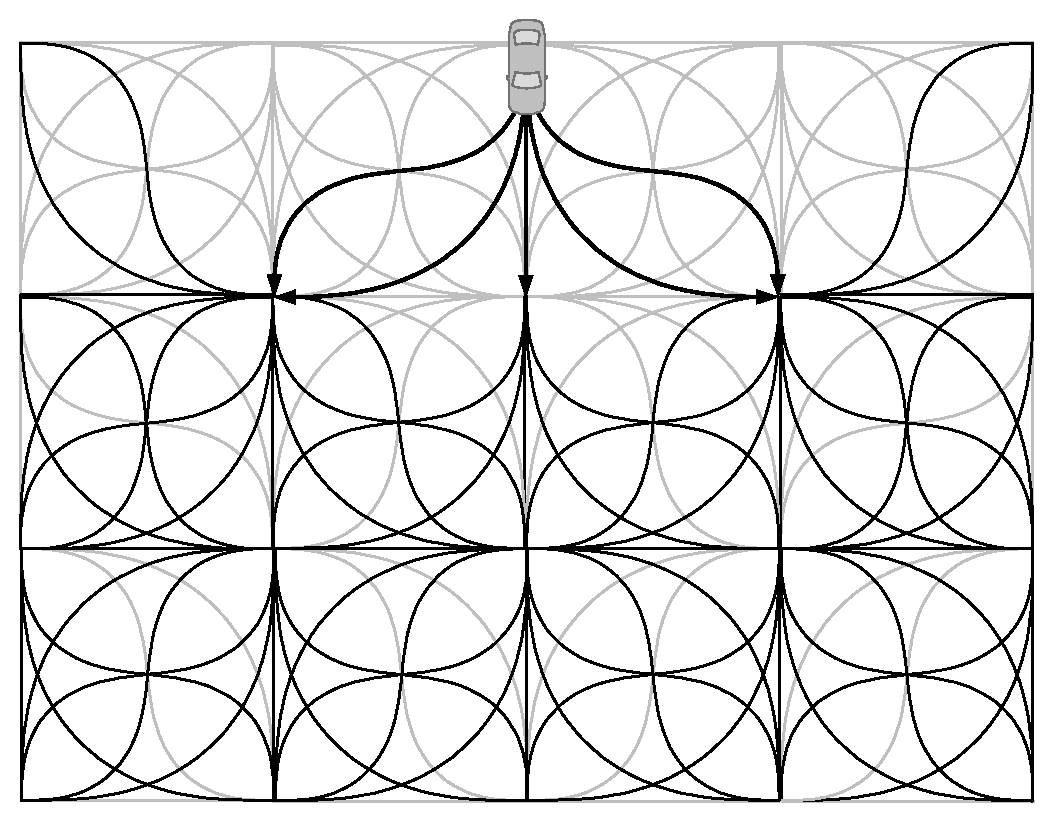
\includegraphics[width=.75\textwidth,clip, trim = 0cm 0cm 0cm 0cm]{7_Lattice.eps}
	\caption[State lattice for unstructured environments]{State lattice for unstructured environments (illustration based on \cite{mcnaughton})}
	\label{fig:lattice}
\end{figure}


%[State lattice for structured environments]
\begin{figure}[h]
\centering
  	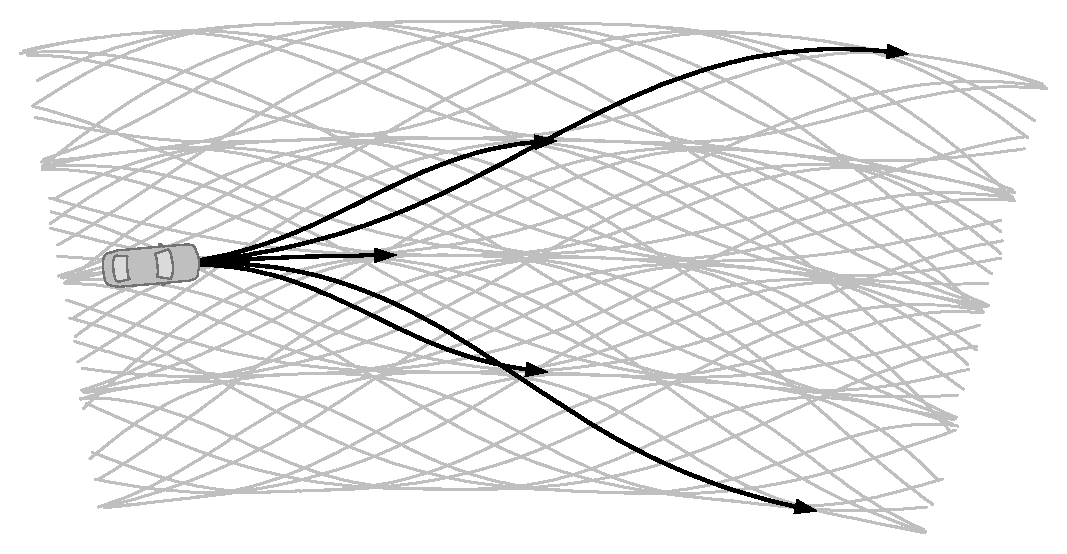
\includegraphics[width=.8\textwidth,clip, trim = 0cm 0cm 0cm 0cm]{7_Lattice_strasse.eps}
	\caption[State lattice for structured environments]{State lattice for structured environments (illustration based on \cite{McNaughton2011diss})}
	\label{fig:lattice_strasse}
\end{figure}



\section{Comparison of the Approaches}\label{S:57.4}


When we compare dynamic programming with direct optimization, we realize that the two approaches possess orthogonal capabilities, see table below.
 Dynamic programming suffers the so-called \emph{curse of dimension} \cite{bellman_DP}%(Bellman 1954)
  meaning that the approach does not scale well with the number of states. Its application is therefore limit to models with few system states (<3-4), and also requires their coarse discretization. Direct optimization, however, can incorporate system models with numerous and continuous system states (>4) and is therefore able to directly feed the system input $\bs{u}(t)$. In turn, direct optimization cannot deal with arbitrary cost functionals due to numerical limitations (local convergence) of the underlying solver. Also, its runtime usually grows exponentially with the number of optimization variables so that the length of the optimization horizon is restricted to a few seconds. As opposed to that, dynamic programming can handle arbitrary costs and will always lead to the global optimum. Furthermore, dynamic programming scales comparably well with the length of the optimization horizon (cf. the linear runtime of the value iteration scheme in  Sect. \ref{57.3.3.2}). 
For complex, farsighted trajectory optimization tasks, the two approaches need to be combined. Dynamic programming will then yield only a “rough long-term plan”, which either serves as the reference trajectory (see e.g.\cite{Ferguson2008, Ferguson2008b, gu2013focused} %(Ferguson et al. 2008a), (Ferguson et al. 2008b) and (Gu et al. 2013)
) and/or provide an initial guess \cite{kang2012online} %(Kang 2012) 
for the locally working direct optimization method. The latter will take a detailed model of the vehicle into account and improves the dynamic programming solution on a reduced optimization horizon to a feasible trajectory (also see  Sect. \ref{57.5}). The optimal state trajectory is either forwarded to a low-level feedback steering/acceleration controller or the optimal input trajectory is directly fed to the vehicle actuators.
Closed form solutions from the calculus of variations are thereby often used to speedup dynamic programming. This can be in the form of a heuristic for an informed search (see e.g. \cite{zieglerIV08}% (Ziegler et al. 2008))
 or a so-called analytical expansions \cite{dolgov2010path},%(Dolgov et al. 2010),
  both of which, roughly speaking, approximate the remaining trajectory and therefore extend the computable optimization horizon, see  Tab.\,\ref{tab:vergleichOpt}.

\begin{center}
\begin{table}[h]
\noindent
\resizebox{\linewidth}{!}{
\begin{tabular}{|l|c|c|c|c|}
\hline
\cline{2-4} Methode
\cellcolor{gray!60} 
& \cellcolor{gray!40} Viele Zustände & \cellcolor{gray!40} Kont.\ Zustände & \cellcolor{gray!40} Glob.\ Optimum & \cellcolor{gray!40} Langer Horizont\\
\hline
%\rowcolor{white!50}
\cellcolor{gray!60} {DP} & $\bs\ominus$ & $\bs\ominus$ & $\bs\oplus$ & $\bs\oplus$ \\
\hline
\cellcolor{gray!60} {DO} & $\bs\oplus$ & $\bs\oplus$ & $\bs\ominus$ & $\bs\ominus$ \\
\hline
\cellcolor{gray!60} {DP + DO} & $\bs\oplus$ & $\bs\oplus$ & $\bs\oplus$ & $\bs\oplus$ \\
\hline
\cellcolor{gray!60} {DP + DO + IO} & $\bs\oplus$ & $\bs\oplus$ & $\bs\oplus$ & $\bs\oplus \bs\oplus$ \\
\hline 
\multicolumn{5}{|c|}{\cellcolor{gray!20} DP: Dynamische Programmierung \quad DO: Direkte Optimierung \quad IO: Indirekte Optimierung}\\
\hline
\end{tabular} }
\caption{Optimierungsmethoden und deren Kombination im direkten Vergleich}
\label{tab:vergleichOpt}
\end{table}
\end{center}



\section{Receding Horizon Optimization}\label{S:57.5}

The receding horizon approach is the gist of \emph{model-predictive control} (MPC, see e.g. \cite{rawlings2000tutorial}),%(Rawlings 2000)),
 which makes a numerical optimization practical for closed loop control. Therein, in each step $t_k$, the OCP is solved on a finite horizon $T$, which calculates the optimal open-loop trajectories $\bar{\bs{x}}^\ast(\tau)$ over $\tau \in [t_k,t_k+T]$, see Fig. \ref{fig:2_mpc_grundidee_u_x}. Only the first part of the optimal control $\bar{\bs{u}}^\ast(\tau)$ is implemented on $\Delta t$. Right in time the new solution is available of the OCP that has been shifted by $\Delta t$. In classical MPC, at each $t_k$ the current plant state is fed back as the new initial state of the OCP. Altogether, this leads to a closed control-loop that anticipates future events, such as input and state saturation, and takes control actions accordingly.
This procedure is completely compatible with trajectory optimization for vehicles. Even more, its replanning mechanism can innately take the limited sensor range and predictability of the other traffic participants into account, which can fundamentally change the OCP from one optimization step to the other. Furthermore, the approach leaves additional degrees of freedom, which can be used to increase the overall robustness of the closed loop system. Firstly, the prediction model may not only include the plant but also the underlying fast low-level feedback or feedforward controllers, which are intended to simplify the resultant optimization model \eqref{equ:opt_systemdynamik}, see also Sect. \ref{57.6}. And secondly, the initial state of the OCP does not necessarily have to be the actual vehicle state but can also be the optimal trajectory of the last step sampled at the current time - or a combination of both. This works as long as the fed-back desired states of the optimal trajectory are tracked by an above-mentioned low-level feedback controller. However, as soon as components of the current vehicle state are used, that show up in the optimization constraints, so-called \emph{slack variables} need to be introduced in the optimization. They transform the otherwise hard inequalities into \emph{soft constraints} as they are referred to in the MPC lingo. This is required as otherwise the slightest disturbance or model uncertainty would ultimately lead to an initial state that the OCP with hard constraints does not have a solution for.
MPC theory offers even more. It also deals with \emph{stability} issues of the closed-loop system such as in \cite{gruene2011nonlinear}.%(Grüne and Pannek 2011).
 More precisely, even for time-invariant system dynamics, constraints, and costs (typical of conventional control problems), the OCP solution changes over time due to the receding horizon, as indicated by Fig. \ref{fig:2_mpc_grundidee_u_x}. In the worst case the differences of the consecutive solutions build up and the system destabilizes. Well-established MPC-schemes therefore propose an augmentation of the cost functional and constraints, e.g., by a special terminal constraint (\emph{invariant set},  \cite{blanchini1999survey})%(Blanchini 1999))
  and cost (\emph{control Lyapunov function}, \cite{gruene2011nonlinear})%(Grüne and Pannek 2011))
   in order to guarantee stability. These schemes can also be transferred to the automotive application. Even more interesting for collision avoidance are the \emph{permanent feasibility} guarantees, which can prevent the sub-optimal short-sighted solutions from “dead ends” also known as \emph{inevitable collision states} (ICS, \cite{fraichard2007short})%(Fraichard 2007))
    in robotics, but this is ongoing research (e.g. \textbf{which???}(Althoff et al. 2012),\cite{Lawitzky2014ICRA}).% (Lawitzky et al. 2014)).




%\section*{Receding Horizon Optimization}
%[Receding horizon optimization]
\begin{figure}[h]
\centering
    \psfrag{x}[lb][lb][1.]{$\bs x(t)$}
		\psfrag{s}[lb][lb][1.]{$\bar{\bs x}^\ast(\tau)$}
		\psfrag{u}[lt][lt][1.]{$\bs u(t)$}
		\psfrag{w}[lt][lt][1.]{$\bar{\bs u}^\ast(\tau)$}
		\psfrag{V}[tr][tr][1.]{past}
		\psfrag{Z}[tl][tl][1.]{future}
		\psfrag{D}[tc][tc][1.]{$\Delta t$}
		\psfrag{T}[tc][tc][1.]{receding horizon $T$}
		\psfrag{t}[tc][tc][1.]{$t,\tau$}
		\psfrag{k}[tc][tc][1.]{$t_k$}
		\psfrag{1}[tc][tc][1.]{$t_{k-1}$}
		\psfrag{2}[tc][tc][1.]{$t_{k-2}$}
		\psfrag{3}[tc][tc][1.]{$t_{k-3}$}
	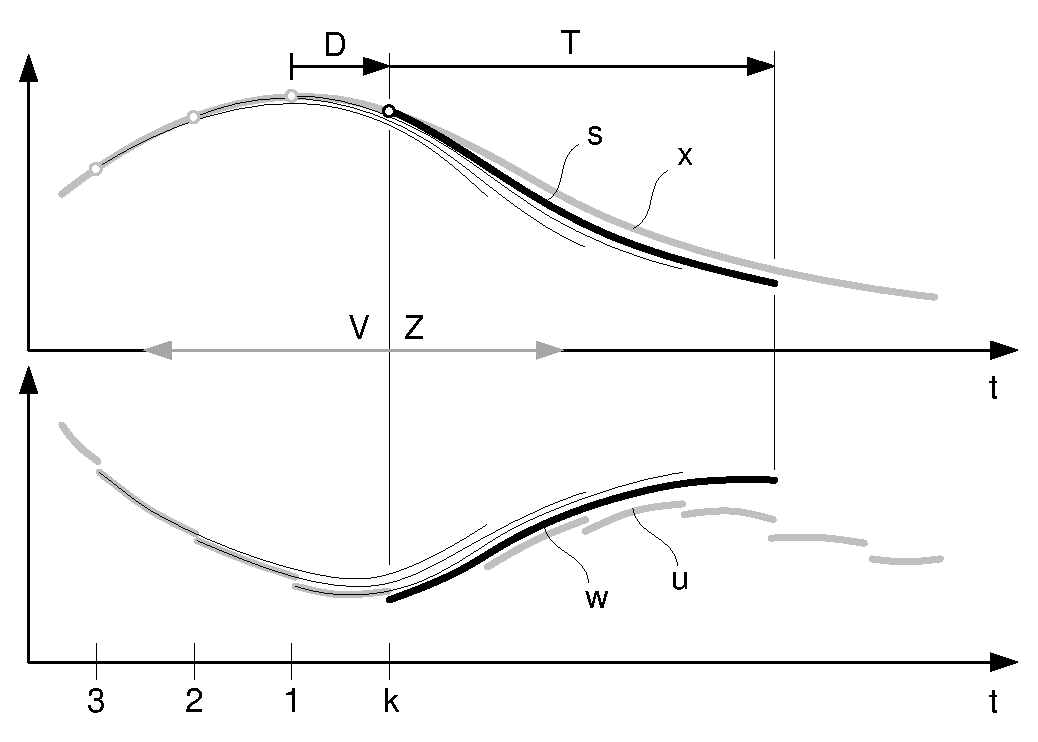
\includegraphics[width=1.\textwidth,clip, trim = 0cm 0cm 0cm 0cm]{2_mpc_grundidee_u_x.eps}
	\caption[Receding Horizon Optimization]{Receding horizon optimization with optimization length $T$, cycle time $\Delta t$, current time step $t_k$, predicted and actual trajectory  $\bar{\bs{x}}^\ast, \bs{x}$ predicted and actual system input $\bar{\bs{u}}^\ast, \bs{u}$}
	\label{fig:2_mpc_grundidee_u_x}
\end{figure}










\section{Conclusion}\label{S:57.6}
Owing to the increase in processing power, computationally intensive optimization algorithms can be executed in real-time in many industrial areas. As automotive electronic control units follow this trend, it is only a matter of time until receding horizon control techniques will emerge in production cars. As has been shown in this chapter, these techniques are most suitable for solving complex trajectory optimization tasks for novel driver assistance systems and automated driving. Based on well-known, elaborated principles we can combine different optimization techniques and implement fast, powerful algorithms with no need to reinvent the wheel.
To surmount the complex integration of numerous safety and comfort functions to a complete driver-friendly unit, an integrated trajectory optimization module is required. Ideally, such a module covers the superset of all emerging use cases. Conventional functions such as emergency braking and lane keeping will then only be special cases within the algorithm.



\newpage
[Finite parameterization of the input]

%

\newpage
 [Physical acceleration limits] \hspace{1.8cm} [System states]
\begin{figure}[h]%
\centering
\begin{minipage}{0.45\textwidth}%
    \psfrag{1}[rb][rb][1.0]{$a_t$}
    \psfrag{2}[cb][cb][1.0]{$a_n$}
    \psfrag{3}[lc][lc][1.0]{$c_t$}
    \psfrag{4}[ct][ct][1.0]{$c_n$}
    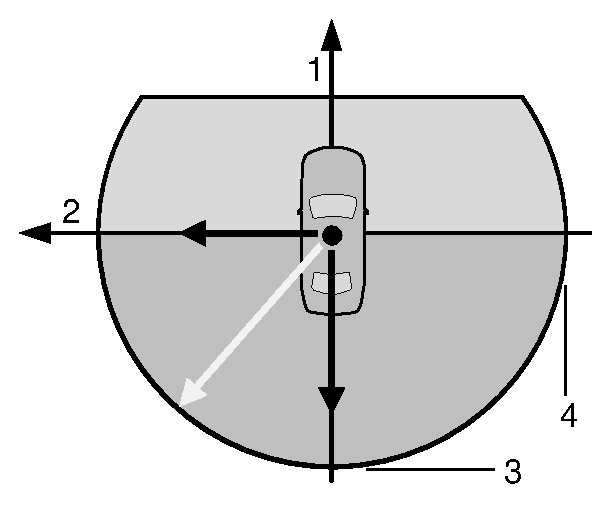
\includegraphics[width=1.0\textwidth,clip, trim = 0cm 0cm 0cm 0cm]{5_KammscherKreis}
    %\caption[Elliptische Näherung der zulässigen Fahrzeugbeschleunigung]{Elliptische Näherung der zulässigen Gesamtfahrzeugbeschleunigung}
    \label{fig:kammscherKreis}
\end{minipage}
\qquad
\begin{minipage}{0.45\textwidth}%
\psfrag{1}[tc][tc][1.0]{$s_r$}
    \psfrag{2}[rb][rb][1.0]{$\kappa_r(s_r)$}
    \psfrag{3}[lb][lb][1.0]{$d_r$}
    \psfrag{4}[rb][rb][1.0]{$[x_1, x_2]$}
    \psfrag{5}[lt][lt][1.0]{$v$}
    \psfrag{6}[c][c][1.0]{$\theta$}
    \psfrag{7}[lt][lt][1.0]{$\theta_r$}
    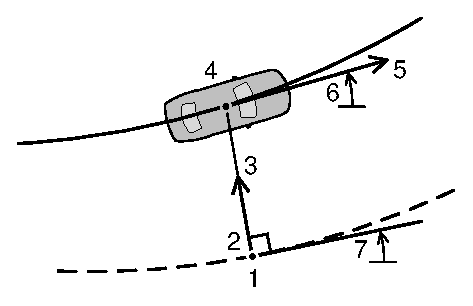
\includegraphics[width=1.0\textwidth,clip, trim = 1.5cm 0cm 0cm 0cm]{5_vehicleAndReferenceCurveStates.eps}
    %\caption[Fahrzeugdynamik entlang einer Referenzkurve]{Systemzustände des vereinfachten Fahrzeugmodells entlang einer Referenzkurve}
    \label{fig:systemStates}
\end{minipage}%
\end{figure}%


	
	
	\newpage
	[Bellman's principle of optimality]
%\section*{Dynamic Programming}
\begin{figure}[h]
	\psfrag{0}[cr][cr][1.0]{$\bs x_0$}
	\psfrag{f}[cl][cl][1.0]{$\bs x_f$}
	\psfrag{t}[ct][ct][1.0]{$t$}
	\psfrag{a}[ct][ct][1.0]{$0$}
	\psfrag{b}[ct][ct][1.0]{$t_f$}
	\psfrag{e}[lb][lb][1.0]{(a)}
	\psfrag{y}[tr][tr][1.0]{$\bs x^\ast(t)$}
	\psfrag{z}[br][br][1.0]{(b)}
	\psfrag{n}[tl][tl][1.0]{(c)}
	\psfrag{x}[cb][cb][1.0]{$\bs x^\ast(t_1)$}
	\psfrag{g}[ct][ct][1.0]{$t_1$}
	\centering
 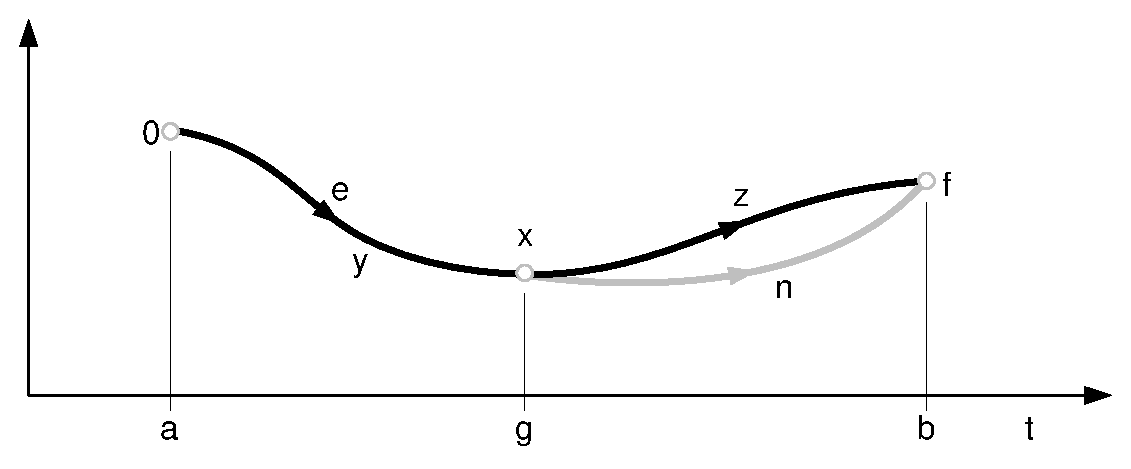
\includegraphics[width=1.0\textwidth,clip, trim = 0cm 0cm 0cm 0cm]{7_Darstellung_Bellmanprinzip.eps}
	%\caption{Zur Verdeutlichung des Bellman'schen Optimalitätsprinzips} 
	\label{fig:Darstellung_Bellmanprinzip}
\end{figure} 

%\newpage 


%\renewcommand{\algorithmiccomment}[1]{// #1}
%\floatname{algorithm}{Algorithmus}






\newpage












